%% ----------------------------------------------------------------
%% GDP.tex
%% ---------------------------------------------------------------- 
\documentclass{desex3}         % Use the GDP Report Style
\usepackage{multicol}
\usepackage{graphicx}
\usepackage{epstopdf}
\usepackage{caption}
\usepackage{subcaption}
%\usepackage{lipsum}% dummy text
%\usepackage{todonotes}
%\usepackage[disable]{todonotes} %uncomment this to disable to do notes
\newcommand{\inote}[1] {\todo[inline]{#1}}
%% \removecolourlinks    % Uncomment this command to remove colour from any links
\newcommand{\cellname}[1] {\clearpage \section{#1} \makebox[\linewidth]{\rule{\textwidth}{0.4pt}}}
\newcommand{\designer}[1] {{\bf Designer: } #1\\}
\newcommand{\celldescription}[1]{{\bf Cell Description: } #1\\}

%\newcommand{\topimages}[3]{
%\begin{multicols}{3}
%\subsection*{Symbol}
%\includegraphics[width=0.5\textwidth,height=4cm,keepaspectratio=true]{#1}
%\subsection*{Dimensions}
%\includegraphics[width=0.5\textwidth,height=4cm,keepaspectratio=true]{#3}
%\end{multicols}
%\subsection*{Circuit Diagram}
%\includegraphics[width=\textwidth,height=3cm,keepaspectratio=true]{#2}
%}

\newcommand{\topimages}[3]{
\begin{figure}[ht!]
        \centering
        \begin{subfigure}[b]{0.5\textwidth}
			\subsection*{Symbol}
                \includegraphics[width=\textwidth]{#1}
        \end{subfigure}%
        ~ %add desired spacing between images, e. g. ~, \quad, \qquad etc.
          %(or a blank line to force the subfigure onto a new line)
        \begin{subfigure}[b]{0.5\textwidth}
				\subsection*{Dimensions}
                \includegraphics[width=\textwidth]{#3}
        \end{subfigure}
		~ %add desired spacing between images, e. g. ~, \quad, \qquad etc.
          %(or a blank line to force the subfigure onto a new line)
        \begin{subfigure}[b]{0.5\textwidth}
				\subsection*{Gate Level Diagram}
                \includegraphics[width=\textwidth]{#2}
        \end{subfigure}
\end{figure}
}
%\newcommand{\topimagesgate}[2]{\begin{multicols}{2}\subsection*{Symbol}\includegraphics[width=\textwidth,height=4cm,keepaspectratio=true]{#1}\subsection*{Dimensions}\includegraphics[width=\textwidth,height=4cm,keepaspectratio=true]{#2}\end{multicols}}

\newcommand{\topimagesgate}[2]{
\begin{figure}[ht!]
        \centering
        \begin{subfigure}[b]{0.5\textwidth}
			\subsection*{Symbol}
                \includegraphics[width=\textwidth]{#1}
        \end{subfigure}%
        ~ %add desired spacing between images, e. g. ~, \quad, \qquad etc.
          %(or a blank line to force the subfigure onto a new line)
        \begin{subfigure}[b]{0.5\textwidth}
				\subsection*{Dimensions}
                \includegraphics[width=\textwidth]{#2}
        \end{subfigure}
\end{figure}
}

\newcommand{\sysverilog}[1]{\subsection*{System Verilog Simulation} \begin{figure}[h!] \centering \includegraphics[width=\textwidth]{#1} \end{figure}}

\newcommand{\acchar}[1]{\subsection*{AC Characteristics}\begin{table}[h!]\centering\begin{tabular}{cc}Signal & Average Delay (ps) \\ \hline\input{#1} \end{tabular}\end{table}}


%% ----------------------------------------------------------------
\begin{document}

\title{Cell Library Databook}

\author{by Team S5\\ H. Lovett (hl13g10) \\ A. J. Robinson (ajr2g10) \\ C. Schepens (cs7g10) \\ M. Wearn (mw20g10)}
%\frontmatter
\maketitle
\cleardoublepage
\tableofcontents
%% ----------------------------------------------------------------
%\mainmatter

\cellname{And2}
\designer{Constantijn Schepens}
\celldescription{A two input AND gate}
\topimages{../and2/symbol.pdf}{../and2/circuitdiagram.jpg}{../and2/blackbox.pdf}

\acchar{../and2/acresults.txt}

\sysverilog{../and2/sv.jpg}


\cellname{BUFFER}
\designer{Ashley Robinson}
\celldescription{A non-inverting buffer}
\topimages{../buffer/symbol.pdf}{../buffer/gateLevel.pdf}{../buffer/blackbox.pdf}

\acchar{../buffer/acresults.txt}

\sysverilog{../buffer/sv.pdf}


\cellname{FULLADDER}
\designer{Martin Wearn}
\celldescription{Adds two bit values and the previous bitsclie carry out, to produce a sum and carry}
\topimages{../fulladder/symbol.png}{../fulladder/circuitdiagram.pdf}{../fulladder/blackbox.pdf}

\acchar{../fulladder/acresults.txt}

\sysverilog{../fulladder/sv.pdf}

\cellname{halfadder}
\designer{Martin Wearn}
\celldescription{Adds two bits to produce a sum and carry}
\topimages{../halfadder/symbol.png}{../halfadder/circuitdiagram.pdf}{../halfadder/blackbox.pdf}

\acchar{../halfadder/acresults.txt}

\sysverilog{../halfadder/sv.pdf}

\cellname{Inverter}
\designer{Henry Lovett}
\celldescription{A basic inverter gate}
\topimages{../inv/symbol.jpg}{../inv/circuitdiagram.jpg}{../inv/blackbox.jpg}

\acchar{../inv/acresults.txt}

\sysverilog{../inv/sv.jpg}

\cellname{leftbuf}
\designer{Henry Lovett}
\celldescription{A start of row buffer cell.}
\topimages{../leftbuf/symbol.pdf}{../leftbuf/circuitdiagram.pdf}{../leftbuf/blackbox.pdf}

\acchar{../leftbuf/acresults.txt}

\sysverilog{../leftbuf/sv.pdf}

\cellname{mux2}
\designer{Constantijn Schepens}
\celldescription{A two input Multiplexor}
\topimages{../mux2/symbol.pdf}{../mux2/circuitdiagram.jpg}{../mux2/blackbox.pdf}

\acchar{../mux2/acresults.txt}

\sysverilog{../mux2/sv.jpg}


\cellname{NAND2}
\designer{Constantijn Schepens}
\celldescription{A two input NAND gate}
\topimagesgate{../nand2/symbol.pdf}{../nand2/blackbox.pdf}

\acchar{../nand2/acresults.txt}

\sysverilog{../nand2/sv.pdf}


\cellname{NAND3}
\designer{Constantijn Schepens}
\celldescription{A three input NAND gate}
\topimagesgate{../nand3/symbol.pdf}{../nand3/blackbox.pdf}

\acchar{../nand3/acresults.txt}

\sysverilog{../nand3/sv.pdf}


\cellname{nand4}
\designer{Constantijn Schepens}
\celldescription{A two input NAND gate}
\topimages{../nand4/symbol.jpg}{../nand4/circuitdiagram.jpg}{../nand4/blackbox.jpg}

\acchar{../nand4/acresults.txt}

\sysverilog{../nand4/sv.jpg}

\cellname{nor2}
\designer{Henry Lovett}
\celldescription{A two input NOR gate}
\topimagesgate{../nor2/symbol.pdf}{../nor2/blackbox.pdf}

\acchar{../nor2/acresults.txt}

\sysverilog{../nor2/sv.jpg}

\cellname{NOR3}
\designer{Henry Lovett}
\celldescription{A three input NOR gate}
\topimagesgate{../nor3/symbol.pdf}{../nor3/blackbox.pdf}

\acchar{../nor3/acresults.txt}

\sysverilog{../nor3/sv.pdf}

\cellname{or2}
\designer{Henry Lovett}
\celldescription{A two input OR gate}
\topimagesgate{../or2/symbol.pdf}{../or2/blackbox.pdf}

\acchar{../or2/acresults.txt}

\sysverilog{../or2/sv.pdf}
%\input{../rdtype/rdtype.tex}

\cellname{RIGHTEND}
\designer{Henry Lovett}
\celldescription{An end of row buffer cell.}
\topimages{../rightend/symbol.pdf}{../rightend/gates.pdf}{../rightend/blackbox.pdf} %no visio for gates as taken from inv

\acchar{../rightend/acresults.txt}

\sysverilog{../rightend/sv.pdf}
%
\cellname{ROWCROSSER}
\designer{Martin Wearn}
\celldescription{A rowcrossing cell}
%\topimages{../rowcrosser/symbol.jpg}{../rowcrosser/circuitdiagram.jpg}{../rowcrosser/blackbox.pdf}

%\acchar{../rowcrosser/acresults.txt}

%\sysverilog{../rowcrosser/sv.jpg}


\cellname{SCANDTYPE}
\designer{Constantijn Schepens}
\celldescription{A scannable D-Type cell}
\topimages{../scandtype/symbol.pdf}{../scandtype/circuitdiagram.pdf}{../scandtype/blackbox.pdf}

\acchar{../scandtype/acresults.txt}

\sysverilog{../scandtype/sv.pdf}


\cellname{scanreg}
\designer{Constantijn Schepens}
\celldescription{A Raw DType cell}
\topimages{../scanreg/symbol.jpg}{../scanreg/circuitdiagram.jpg}{../scanreg/blackbox.jpg}

\acchar{../scanreg/acresults.txt}

\sysverilog{../scanreg/sv.jpg}
%\input{../smux2/smux2.tex}
%\input{../smux3/smux3.tex}
%
\cellname{TIEHIGH}
\designer{Martin Wearn}
\celldescription{A tie to Vdd cell}
%\topimages{../tiehigh/symbol.jpg}{../tiehigh/circuitdiagram.jpg}{../tiehigh/blackbox.pdf}

%\acchar{../tiehigh/acresults.txt}

%\sysverilog{../tiehigh/sv.jpg}

%
\cellname{tielow}
\designer{Martin Wearn}
\celldescription{A tie to GND cell}
\topimages{../tielow/symbol.jpg}{../tielow/circuitdiagram.jpg}{../tielow/blackbox.pdf}

\acchar{../tielow/acresults.txt}

\sysverilog{../tielow/sv.jpg}
\newpage
\section{Rowcrosser} %\makebox[\linewidth]{\rule{\textwidth}{0.4pt}
{\bf Designer: } Martin Wearn\\
{\bf Cell Description: } A row crossing cell.\\
\subsection*{Dimensions}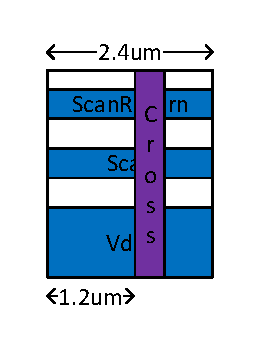
\includegraphics[width=\textwidth,height=4cm,keepaspectratio=true]{../rowcrosser/blackbox.pdf}

\section{Tie High} %\makebox[\linewidth]{\rule{\textwidth}{0.4pt}
{\bf Designer: } Martin Wearn\\
{\bf Cell Description: } A tie to Vdd cell.\\
\subsection*{Dimensions}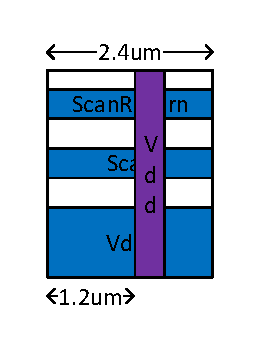
\includegraphics[width=\textwidth,height=4cm,keepaspectratio=true]{../tiehigh/blackbox.pdf}

\section{Tie Low} %\makebox[\linewidth]{\rule{\textwidth}{0.4pt}
{\bf Designer: } Martin Wearn\\
{\bf Cell Description: } A  tie low cell.\\
\subsection*{Dimensions}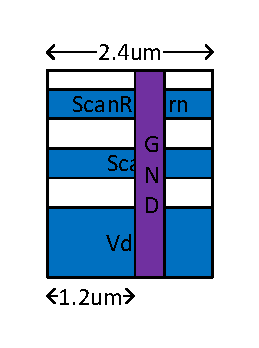
\includegraphics[width=\textwidth,height=4cm,keepaspectratio=true]{../tielow/blackbox.pdf}

\cellname{TRISBUF}
\designer{Ashley Robinson}
\celldescription{A tristate buffer}
\topimages{../trisbuf/symbol.pdf}{../trisbuf/gateLevel.pdf}{../trisbuf/blackbox.pdf}

\acchar{../trisbuf/acresults.txt}

\sysverilog{../trisbuf/sv.pdf}


\cellname{xor2}
\designer{Ashley Robinson}
\celldescription{A two input xor gate}
\topimages{../xor2/symbol.pdf}{../xor2/gateLevel.pdf}{../xor2/blackbox.pdf}

\acchar{../xor2/acresults.txt}

\sysverilog{../xor2/sv.pdf}


\appendix
\clearpage
\section{Appendix A}

\subsection{Team Management}

\subsubsection{Justification of the Division of Labour}

The four major cells were divided between the team as recommended in the specification.
It was decided to also attempt the optional cells for teams of four.
An extra person in a team of five would be in charge of designing the halfadder and xor2.
The halfadder was assigned to the team member designing the fulladder as their expertise was greater for designing adder cells.
The xor2 cell was assigned to the team member designing the rdtype as this cell was assumed less time consuming than the two other sets of major cells.
The remaining cells were grouped and divided among the teams as shown in Table~\ref{tab:cells}.

\begin{table}[h]
   \centering
    \begin{tabular}{| p{4.5cm} | p{6.5cm} |}
    \hline
      \textbf{Cell Groupings} & \textbf{Reasoning}\\ \hline
      and2, and2, nand3, nand4  &	Nands and Ands are similar in design.\\ \hline
      buffer, trisbuf  &	Buffers are similar in design.\\ \hline
      inverter, nor2, nor3, or2   &	 Nors and Ors similar in design. Inverter is a simple cell assigned to distribute load.\\ \hline
      rowcrosswer, tiehigh, tielow &	Low complexity cells assigned to team member tasked with designing both adders.\\ \hline
    \end{tabular}
    \caption{Cell design groupings and reasoning}
    \label{tab:cells}
\end{table}

\subsubsection{Version Control}
The Git revision control system was used throughout the project to facilitate collaborative working.
GitHub is a web-based hosting service for git. 
This was used to share files, allocate work and track bugs.

\subsubsection{Process automation}
The team produced a number of scripts to improve productivity by automating processes such extraction from magic, design simulation and consistency checking.
Using Latex allowed the databook compilation to also be automated as separate files for each cell were stored in the hierarchy of folders.   
This way each designer could add their own files to the data book independently.



\clearpage
\subsection{Division of Labour}
\begin{table}[htb!]
\begin{tabular}{|p{1cm}|c|c|c|c|c|}\hline
&Task & \multicolumn{4}{|c|}{Percentage Effort on Each Task (\%)} \\ \hline
& ECS ID 						& mw20g10 & cs7g10 & ajr2g10 & hl13g10 \\ \hline
1&RDTYPE						&	0	&	0	&	100	&	0	\\ \hline
2&SMUX2							&	0	&	100	&	0	&	0	\\ \hline
3&SMUX3							&	0	&	100	&	0	&	0	\\ \hline
4&MUX2							&	0	&	100	&	0	&	0	\\ \hline
5&FULLADDER					&	100	&	0	&	0	&	0	\\ \hline
6&HALFADDER					&	100	&	0	&	0	&	0	\\ \hline
7&XOR2							&	0	&	0	&	100	&	0	\\ \hline
8&INV								&	0	&	0	&	0	&	100	\\ \hline
9&NAND2							&	0	&	100	&	0	&	0	\\ \hline
10&NAND3						&	0	&	100	&	0	&	0	\\ \hline
11&NAND4						&	0	&	100	&	0	&	0	\\ \hline
12&NOR2							&	0	&	0	&	0	&	100	\\ \hline
13&NOR3							&	0	&	0	&	0	&	100	\\ \hline
14&AND2							&	0	&	100	&	0	&	0	\\ \hline
15&OR2							&	0	&	0	&	0	&	100	\\ \hline
16&TRISBUF					&	0	&	0	&	100	&	0	\\ \hline
17&BUFFER						&	0	&	0	&	100	&	0	\\ \hline
18&LEFTBUF					&	0	&	0	&	0	&	100	\\ \hline
19&RIGHTEND					&	0	&	0	&	0	&	100	\\ \hline
20&TIEHIGH					&	100	&	0	&	0	&	0	\\ \hline
21&TIELOW						&	100	&	0	&	0	&	0	\\ \hline
22&ROWCROSSER				&	100	&	0	&	0	&	0	\\ \hline
23&SCANDTYPE				&	0	&	0	&	0	&	0	\\ \hline
24&SCANREG					&	0	&	0	&	0	&	0	\\ \hline
25&Verilog Simulation				&	20	&	20	&	20	&	40	\\ \hline
26&HSpice Characterization	&	20	&	40	&	20	&	20	\\ \hline
27& Final Report (words)		&	30	&	20	&	30	&	20	\\ \hline
28& Final Report (figures)	&	25	&	25	&	25	&	25	\\ \hline
& OVERALL EFFORT 						&	23	&	23	&	23	&	31	\\ \hline
& Signature: 								& 		& 		& 		&		\\ \hline
\end{tabular}
\end{table}

\clearpage
\section{Design Detail}
\renewcommand{\cellname}[1] {\newpage \subsection{#1} \makebox[\linewidth]{\rule{\textwidth}{0.4pt}}}
\newcommand{\stickdiagram}[1]{\subsubsection*{Stick Diagram} \includegraphics[width=\textwidth,height=12cm,keepaspectratio=true]{#1}}
\newcommand{\transistor}[1]{\subsubsection*{Transistor Level Circuit Diagram} \includegraphics[width=0.5\textwidth,keepaspectratio=true]{#1}}

\cellname{FULLADDER}
\designer{Martin Wearn}
\celldescription{Adds two bit values and the previous bitslice carry out, to produce a sum and carry}

This cell is designed for the addition of two single bits taking into account the carry out of the previous bitslice.
It is a key element for the design and construction of larger ALU modules and can also implement a subtract function if used with an XOR gate.
The truth table for this cell can be seen in the table below.

\begin{tabular}{| c | c | c || c | c |}
\hline
A & B & Cin & S & Cout \\ \hline
0 & 0 & 0   & 0 & 0    \\
0 & 0 & 1   & 1 & 0    \\
0 & 1 & 0   & 1 & 0    \\
0 & 1 & 1   & 0 & 1    \\
1 & 0 & 0   & 1 & 0    \\
1 & 0 & 1   & 0 & 1    \\
1 & 1 & 0   & 0 & 1    \\
1 & 1 & 1   & 1 & 1    \\ \hline
\end{tabular}

A compound gate structure is used to minimise the number of transistors used within the design. 
Layout of transistors has been done using a euler paths combined with gate matrix design.
The first compound gate, for sum output, had a euler path of A-A-B-Cin-X-Cin-B. Whereas the second compund gate, for carry out, has a euler path of A-A-B-Cin-B. Where X was the inverted Cout connection.
These were then laid out as two diagrams, each with a single line of diffusion for PMOS and NOMS transistors.
Since the euler paths were identical, but with a gap in carry out between Cin and B, they could be combined into same stick diagram. Placing the carry out lines between the sum lines and including the two output inverters in the same rows as the compound gate they are attached to.
After this, futher tweaks were made to optimise the routing for minimum space occupied by cell. 
This gave a final design consisting of two lines of diffusion and 9 polysilicon columns. 

\stickdiagram{../fulladder/stickdiagram.pdf}
\acchar{../fulladder/acresults.txt}
\transistor{../fulladder/transistorcd.pdf}
\spicesim{../fulladder/hspiceColor.png}

Measure commands were used to determine propagation delays from each input to each output. These measured the time from an input going high to an output going high or low, and the time from an input going low to an output going high or low. 
Averages were then taken to determine the propagation time between each input changing and the correct value being expected at an output. 

\cellname{HALFADDER}
\designer{Martin Wearn}
\celldescription{Adds two bits to produce a sum and carry}

This cell is designed for the addition of two single bits to produce their sum and carry out. 
It can be used along the edge of a row of full adders since there will be no carry in to consider. Where possible, this should be used instead of a full adder because of the space saving benefits and circuit simplification. 
The truth table for this cell can be seen in the table below.

\begin{tabular}{| c | c || c | c |}
\hline
A & B &  S & C \\ \hline
0 & 0 &  0 & 0 \\
0 & 1 &  1 & 0 \\
1 & 0 &  1 & 0 \\
1 & 1 &  0 & 1 \\ \hline
\end{tabular}

A combination of a compound gate and a nand gate was used to minimise the number of transistors used within the design.
This was followed through to transistor level design but not the stick diagram. Seperate gates with an additional inverter was used to simplify gate matrix design and remove the risk of earlier issues with compound gate design reoccuring within this cell.
The gate matrix layout used places one NOR, NAND and NOT on one row, and the other NAND and two NOT's on the second row. Metal routing around the cell occupied very little space compared to the full adder, so no optimisation was needed.
The resultant final design has two additional transistors than originally planned and one additional polysilicon column. 
It has two lines of diffusion for each of the NMOS and PMOS transistors and 6 polysilicon columns. 

\stickdiagram{../halfadder/stickdiagram.pdf}
\acchar{../halfadder/acresults.txt}
\transistor{../halfadder/transistorcd.pdf}
\spicesim{../halfadder/hspiceColor.png}

Measure commands were used to determine propagation delays from each input to each output. These measured the time from an input going high to an output going high or low, and the time from an input going low to an output going high or low. 
Averages were then taken to determine the propagation time between each input changing and the correct value being expected at an output. 

\cellname{LEFTBUF}
\designer{Henry Lovett}
\celldescription{A start of row buffer cell.}

This cell is to be placed at the beginning of each row of cells. 
The purpose of this cell is to buffer the \textit{Clock, nReset} and \textit{Test} signals to attempt to eliminate skew of the signals.
They also cater for the scan path in the circuit by routing and buffering the signal.

This cell contains 3 large buffers, each made up of 4 stages.
The gain of the stages are gradually increased, relative to the first. 
The transistors were folded to reduce the vertical height of the cell. 
The total, and folded sizes of the transistors are seen in the table below.

\begin{table}[htb!]
\centering
\begin{tabular}{c|cccc}
Stage						&	1				&	2		&	3		&	4 \\ \hline
Gain 						& 	1 				& 	2.7 	& 	7.3 	& 	20 \\
$W_n$ unfolded 	($\mu m$) 	&	1.0 			& 	2.7 	& 	7.3 	& 	20 \\
$W_p$ unfolded	($\mu m$)	& 	2.9				& 	7.85 	& 	21.2 	& 	58 \\
$W_n$ folded	($\mu m$)	&	$1 \times 1.0$ 	& 	$1 \times 2.7$ 		& 	$1 \times 7.3$ 		& 	$2 \times 10.0$ \\
$W_p$ folded	($\mu m$)	&	$1 \times 2.9$ 	& 	$1 \times 7.85$ 	& 	$2 \times 10.6$ 	& 	$4 \times 14.5$ \\
\end{tabular}
\end{table}

\stickdiagram{../leftbuf/stickdiagram.pdf}
\acchar{../leftbuf/acresults.txt}
\transistor{../leftbuf/transistorcd.pdf}
\spicesim{../leftbuf/hspiceColor.png}
%override of default
%\subsubsection*{HSpice Simulation}
%\begin{figure}[ht!]
%        \centering
%        \begin{subfigure}[b]{0.5\textwidth}
%                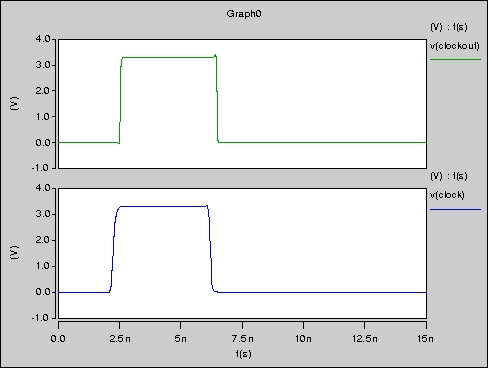
\includegraphics[width=\textwidth]{../leftbuf/hspiceClockColor.png}
%%        \end{subfigure}%
 %       ~ %add desired spacing between images, e. g. ~, \quad, \qquad etc.
 %         %(or a blank line to force the subfigure onto a new line)
 %       \begin{subfigure}[b]{0.5\textwidth}
 %               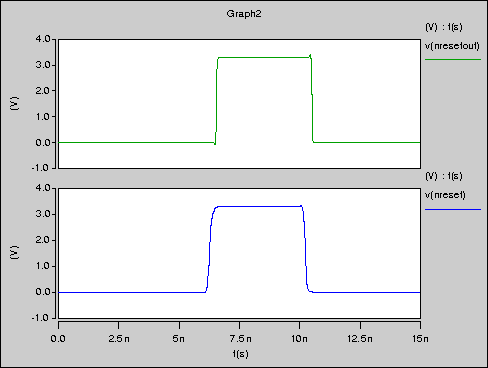
\includegraphics[width=\textwidth]{../leftbuf/hspiceNResetColor.png}
 %       \end{subfigure} 
%		~ %add desired spacing between images, e. g. ~, \quad, \qquad etc.
%          %(or a blank line to force the subfigure onto a new line)
%        \begin{subfigure}[b]{0.5\textwidth}
%                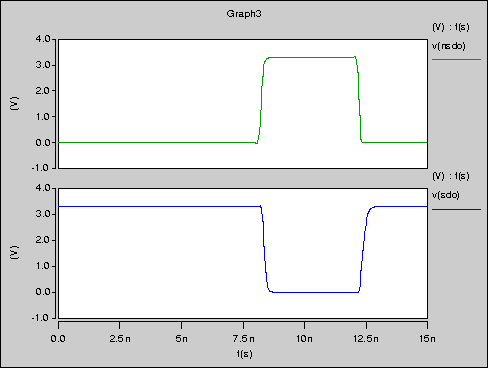
\includegraphics[width=\textwidth]{../leftbuf/hspiceSDOColor.png}
%        \end{subfigure} 
%		~ %add desired spacing between images, e. g. ~, \quad, \qquad etc.
%          %(or a blank line to force the subfigure onto a new line)
%        \begin{subfigure}[b]{0.5\textwidth}
%                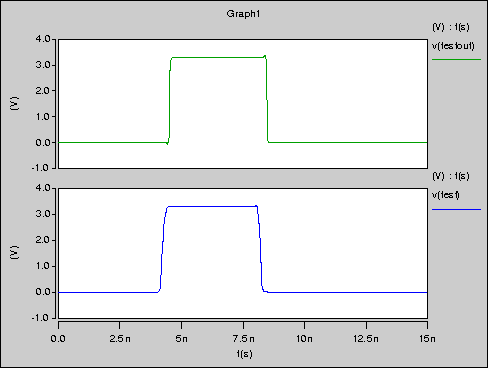
\includegraphics[width=\textwidth]{../leftbuf/hspiceTestColor.png}
%        \end{subfigure}
%\end{figure}

\cellname{rdtype}
\designer{Ashley Robinson}
\celldescription{Raw Dtype}

This gate matrix design was optimised by arranging polysilicon columns to allow as many transistors to fit on a row as possible.
Three rows of PMOS transistors and four rows of NMOS transistors make up cell.
Routing power rails up both sides of the matrix allowed the design to be further compressed.
The D input on the middle left was intentionally not surrounded leaving only metal1 to reroute when it came to dimension matching.

\stickdiagram{../rdtype/stickdiagram.pdf}
\transistor{../rdtype/transistorcd.pdf}

%TO DO : Results of loaded simulation bits

\cellname{SMUX2}
\designer{Constantijn Schepens}
\celldescription{A 2 input scannable multiplexer, intended to be connected to a
raw D-type to create a scannable D-type.}

A single Euler path was used when laying out this cell, before taking into
account inverters. The Euler path (T-nT-D-S) was designed such that the output was all the
way on the right side such that it could connect directly to the D input of the
raw D-type. Once this was done the required internal inverters were added in by
creating a gate matrix design. 

\stickdiagram{../smux2/stickdiagram.pdf}
\acchar{../smux2/acresults.txt}
\transistor{../smux2/transistorcd.pdf}
\spicesim{../smux2/hspiceColor.png}
\cellname{smux3}
\designer{Constantijn Schepens}
\celldescription{A 3 input scannable multiplexer, intended to be connected to a
raw D-type to create a scannable register.}

A similar approach was taken for the layout of this cell as for the smux2.
Initially inverters were excluded and a single Euler path
(D-Load-nTest-Test-SDI-nLoad-Q) was found that both
kept M and Q as close to the right side as possible (to connect to the raw
D-type) and  kept the Test/Load nearest to their inverted partners for easy wiring.
For the internal inverter placement multiple layouts were trialed to find the
most efficient one, that also allowed all the internal wiring to be done with
metal 1 exclusively(to reduce the number of vias).

\stickdiagram{../smux3/stickdiagram.pdf}
\transistor{../smux3/transistorcd.pdf}

%TO DO : Results of loaded simulation bits

\cellname{xor2}
\designer{Ashley Robinson}
\celldescription{A 2 input XOR gate.}

Compound gate routed using an Euler path.

\stickdiagram{../xor2/stickdiagram.pdf}
\acchar{../xor2/acresults.txt}
\transistor{../xor2/transistorcd.pdf}
\spicesim{../xor2/hspice.png}


\end{document}
%% ----------------------------------------------------------------
